\section{Optimizing software}
\subsection{Coherence misses}
    \begin{tcolorbox}[vert]
        Coherence adds extra misses when two cores access the same cache line, then there is two types of coherence misses:
        \begin{itemize}[left=10pt, label=\textbullet]
            \item \important{True sharing}: the producer/consumer communication when processors read and write the same variable. 
            \item \important{False sharing}: processors updating different data which are placed in the same cache block.
        \end{itemize}
    \end{tcolorbox}
    \textbf{True sharing, histogram example:}
    \begin{tcolorbox}[gris]
        We have an input text and we want to count the occurrences of each different characters in the text. We'll use OpenMP to divide the work across threads.
    \end{tcolorbox}
    \begin{codeCenter}
    \begin{Ccode}
int histogram[N_BUCKETS];
int in_data[INPUT_SIZE];

#pragma omp parallel for shared (in_data, histogram)
for(int i = 0; i < INPUT_SIZE;i++) {
    unsigned bucket = calc_hist(in_data[i]);

    #pragma omp critical
    histogram[bucket]++;
}
    \end{Ccode}
    \end{codeCenter}
    Then, there is true sharing when processors modify the histogram \lstinline!histogram['a']++;!. To avoid this, we have to preserve correct value. Then we can \begin{codeCenter}
    \begin{Ccode}
int histogram[N_BUCKETS];
int tmp_hist[N_THREADS][N_BUCKETS];
int in_data[INPUT_SIZE];

// Repartition loop
#pragma omp parallel for shared (in_data, tmp_hist)
for(int i = 0; i < INPUT_SIZE;i++) {
    int tid = omp_get_thread_num();
    unsigned bucket = calc_hist(in_data[i]);
    tmp_hist[tid][bucket]++;
}

// Merge loop
#pragma omp parallel shared (tmp_hist, histogram)
for(int i = 0; i < N_BUCKETS; i++) {
    int tid = omp_get_thread_num();
    #pragma omp critical
    histogram[i] += tmp_hist[tid][i];
}
    \end{Ccode}
    \end{codeCenter}
    \begin{remark}{Remark}
        In the code, \lstinline!shared (x, y)! tells OpenMP that all threads should see and access the same variable in memory (shared memory communication).
    \end{remark}
    In the first code, we have \lstinline!INPUT_SIZE! times the critical section and the read/write to the histogram. In the second one, we have \lstinline!N_BUCKETS! times the number of threads, then if the size of the input is way bigger than the number of buckets times the number of threads, we eliminate a lot of critical sections and true sharing. \\
    Here is just an alternative of the merge loop that eliminating all critical sections, but every thread accesses a fraction of everyone's histogram.
        \begin{codeCenter}
        \begin{Ccode}
// Merge loop
#pragma omp parallel for shared (tmp_hist, histogram)
for(int i = 0; i < N_BUCKETS; i++) {
    int tid;
    for (tid = 0; tid < omp_get_num_threads(); tid++) {
        histogram[i] += tmp_hist[tid][i];
    }
}
        \end{Ccode}
        \end{codeCenter}


    \textbf{False sharing, odd numbers example:}
    \begin{codeCenter}
    \begin{Ccode}
int counters[NTHREADS];
int in_data[INPUT_SIZE];

#pragma omp parallel for shared (in_data,counters)
for(int i = 0; i < INPUT_SIZE;i++) {
    int tid = omp_get_thread_num();
    
    if(in_data[i] % 2) {
        counters[tid]++;
    }
}
    \end{Ccode}
    \end{codeCenter}
    \begin{tcolorbox}[gris]
        Nowadays, cache line are 64 byte in general, then it can store the four \lstinline!int! on the same cache line. So every time a core update its counter value, it invalidate every other cache line, this is false sharing!
    \end{tcolorbox}
    
    \begin{center}
    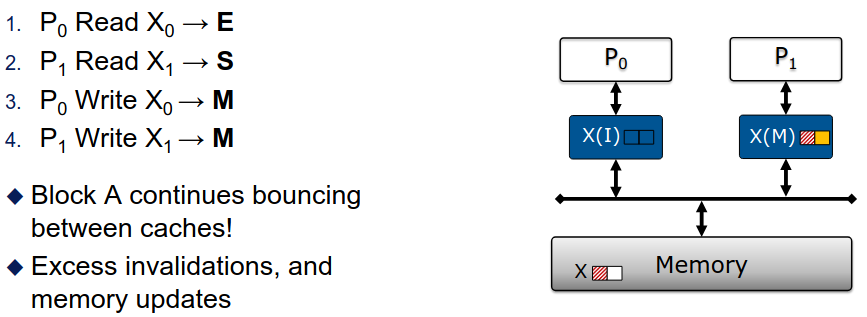
\includegraphics[width=9cm]{images/16.png}
    \end{center}
    The solution here is to add padding, so the int are not on the same cache block anymore (e.g. 64 byte cache block line, a \lstinline!int! is 4 byte, then we add a padding of 60 bytes).
    \begin{codeCenter}
    \begin{Ccode}
typedef struct {
    unsigned _c;
    unsigned _padding[ BLK_SIZE/ UNSIG_SIZE - 1];
} PaddedCounter;
PaddedCounter counters[NTHREADS];

#pragma omp parallel for
{
    ...
    counters[tid]._c++;
}
    \end{Ccode}
    \end{codeCenter}
    \begin{tcolorbox}[violet]
        We saw that eliminating false sharing take a lot of space, so the capacity and conflict misses increases. Then, the bigger the cache is, the less the padding is efficient to reduct global misses.
    \end{tcolorbox}
    \begin{center}
    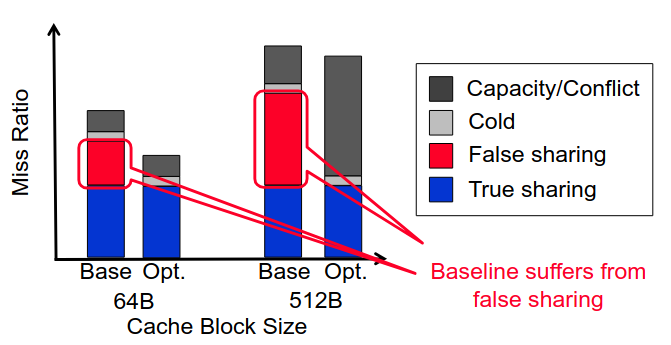
\includegraphics[width=9cm]{images/17.png}
    \end{center}
    \textbf{Block locality:}\\
    The locality of caches can be a problem in a program that, for example, multiply matrices, because we read the first matrix vertically and the second one horizontally.
    \begin{center}
    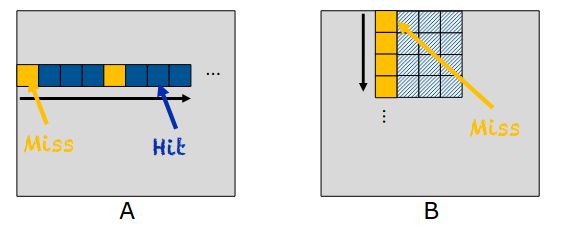
\includegraphics[width=9cm]{images/18.png}
    \end{center}
    Arrays are too large to fit in caches, then if we want to calculate $A \cdot  B = C$, for every element of C if A and B are of size NxN, we'll have $1+N\left[\frac{4}{\text{cache line size}}\right]+N$ misses! Then for the whole calculation, we obtain $\left(N^3\left(1+c\right)+N^2\right)$ which is $O\left(N^3\right)$ misses (where $c =\frac{\text{element size}}{\text{cache line size}}$).\\
    \hypertarget{matrix}{}
    \begin{image}{To avoid this, we can do blocking. \\ Then, for the whole array, we have to create $\left(\frac{N}{n}\right)^2$ blocks and they have $2\cdot \left[\frac{4\cdot n}{\text{cache line size}}\right]$ misses, so finally we have $O\left(N^2\right)$ misses.}
        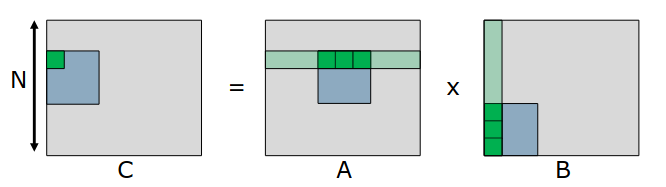
\includegraphics[width=9cm]{images/19.png}
    \end{image}
\subsection{Work distribution and scheduling}
    \begin{tcolorbox}[violet]
        OpenMP is a join/fork model where fork creates a team of parallel threads and join, synchronize and terminate threads  at the end of parallel region. But fork and join comes with an overhead.
    \end{tcolorbox}
    \begin{image}{For a code like this, if the loop has too few iterations, the fork and join overhead is bigger than the savings made by the parallel execution. There is no need to parallelize the loop.}
        \begin{codeCenter}
        \begin{Ccode}
#pragma omp parallel for
for(i = 0; i < n; i++)
        \end{Ccode}
        \end{codeCenter}
    \end{image}
    We can use the \lstinline!if! clause to resolve this: \lstinline!#pragma omp parallel for if(n > 5000)!.\\
